	%You can delete all the comments after you have finished your document
%this sets up the defaults for the documents, 12pt font and A4 size. The article type sets this up as such as opposed to letter or memo.

%for the finer points LaTeX see https://en.wikibooks.org/wiki/LaTeX or http://tex.stackexchange.com/

\documentclass[12pt,a4paper,oneside]{article}
\usepackage{titlesec} %these are how we import packages, one helps set up footers and title layout
\setcounter{secnumdepth}{4}
\usepackage{fancyhdr}

% !TEX TS-program = pdflatex
% !TEX encoding = UTF-8 Unicode
\usepackage[utf8]{inputenc} % set input encoding (not needed with XeLaTeX)

\usepackage{graphicx} % support the \includegraphics command and options

\usepackage[parfill]{parskip} % Activate to begin paragraphs with an empty line rather than an indent

%%% PACKAGES
\usepackage{cite} % for IEEE style number references
\usepackage{setspace} % for control over line spacing
\onehalfspacing
\usepackage{booktabs} % for much better looking tables
\usepackage{array} % for better arrays (eg matrices) in maths
\usepackage{paralist} % very flexible & customisable lists (eg. enumerate/itemize, etc.)
\usepackage{verbatim} % adds environment for commenting out blocks of text & for better verbatim
\PassOptionsToPackage{hyphens}{url}\usepackage{hyperref} % adds \url command for hyperlinks in text, makes them black and allows wrapping on url hyphens
\hypersetup{
	colorlinks=false,
	linkcolor=black,
	filecolor=black,      
	urlcolor=black,
}
%\usepackage[multiple]{footmisc}
\usepackage{subfig} % make it possible to include more than one captioned figure/table in a single float
%\usepackage[authoryear]{natbib} % adds APA referencing style to standard LaTeX bibliography support
\usepackage[toc,page]{appendix}
% These packages are all incorporated in the memoir class to one degree or another...

%header and footer settings
\pagestyle{fancyplain}
\fancyhf{}
\renewcommand{\headrulewidth}{0.5pt}
\renewcommand{\footrulewidth}{0.5pt}
\setlength{\headheight}{15pt}
\fancyhead[L]{Beej Persson - 40183743}
\fancyhead[R]{SOC10101 Honours Project}
\fancyfoot[L]{}
\fancyfoot[C]{\thepage}
\pagenumbering{roman}

%set better section layout

\makeatletter
\renewcommand\paragraph{\@startsection {paragraph}{1}{0mm} % name, level, indent
	                           {3pt plus 2pt minus 1pt} % before skip
	                           {3pt plus 0pt} % after skip
	                           {\normalfont}}
\makeatother
\makeatletter
\renewcommand\subsubsection{\@startsection {subsubsection}{1}{0mm} % name, level, indent
	                           {3pt plus 2pt minus 1pt} % before skip
	                           {3pt plus 0pt} % after skip
	                           {\normalfont\bfseries}}
\makeatother
\makeatletter
\renewcommand\subsection{\@startsection {subsection}{1}{0mm} % name, level, indent
                               {3pt plus 2pt minus 1pt} % before skip
                               {3pt plus 0pt} % after skip
                               {\large\bfseries}}
\makeatother
\makeatletter
\renewcommand\section{\@startsection {section}{1}{0mm} % name, level, indent
                               {4pt plus 2pt minus 1pt} % before skip
                               {4pt plus 0pt} % after skip
                               {\Large\bfseries}}
\makeatother


%this starts the document
\begin{document}

%you can import other documents into your main one, these layout the Title and Declarations on its own page.
%you might need to change these to \ if your on Microsoft Windows.
\begin{singlespace}	
\newcommand{\HRule}{\rule{\linewidth}{0.5mm}}

\begin{titlepage}
	\begin{center}

	\HRule \\[0.4cm]
    	{\Large \bfseries Real-World Object Capture in a \\ Mixed Reality Environment\par}
	\vspace{0.2cm}
	\HRule \\[1.5cm]

	
    	\vspace{3cm}
	\begin{minipage}{0.4\textwidth}
	\begin{center} \large
        \emph{}\\
        	Beej Persson - 40183743
				
   	 \end{center}
    	\end{minipage}
	
	\vspace{2cm}
    	\begin{minipage}{1\textwidth}
    	\begin{center} \large
        
		Submitted in partial fulfilment of \\
		the requirements of Edinburgh Napier University \\
		for the Degree of \\
        	BSc (Hons) Games Development
    	\end{center}
    	\end{minipage}

    	\vfill

    	% Bottom of the page
	\begin{minipage}{1\textwidth}
    	\begin{center} \large
		School of Computing
    	\end{center}
    	\end{minipage}
	
	\vspace{1cm}
    	{\large \today}


	\end{center}
\end{titlepage}
%{\large Submitted in partial fulfilment of the requirements of Edinburgh Napier University for the Degree of }

\section*{Authorship Declaration}
\vspace{0.5cm}
\begin{flushleft}
I, Beej Persson, confirm that this dissertation and the work presented in it are my own achievement.\newline

Where I have consulted the published work of others this is always clearly attributed;\newline

Where I have quoted from the work of others the source is always given. With the exception of such quotations this dissertation is entirely my own work;\newline

I have acknowledged all main sources of help; \newline

If my research follows on from previous work or is part of a larger collaborative research project I have made clear exactly what was done by others and what I have contributed myself;\newline

I have read and understand the penalties associated with Academic Misconduct.\newline

I also confirm that I have obtained informed consent from all people I have involved in the work in this dissertation following the School's ethical guidelines.\newline
\end{flushleft}

\begin{flushleft} \large
\emph{Signed:} \\
\end{flushleft}

\vspace{.5cm}

\begin{flushleft} \large
\emph{Date:} \\
\end{flushleft}

\vspace{.5cm}

\begin{flushleft} \large
\emph{Matriculation no: }  \\
\end{flushleft}
\pagebreak

\section*{Data Protection Declaration}
\vspace{0.5cm}
\begin{flushleft}
Under the 1998 Data Protection Act, The University cannot disclose your grade to an unauthorised person. However, other students benefit from studying dissertations that have their grades attached. \newline

\vspace{0.5cm}

Please sign your name below one of the options below to state your preference.\newline
\vspace{0.5cm}

The University may make this dissertation, with indicative grade, available to others.\newline
\vspace{3cm}


The University may make this dissertation available to others, but the grade may not be disclosed.\newline
\vspace{3cm}


The University may not make this dissertation available to others.\newline
\end{flushleft}


\pagebreak
\end{singlespace}
%LaTeX let you define the abstract separately so it wont get sucked into the main document.
\begin{abstract}
Mixed reality is an increasingly popular technology due to its nature of combining real and virtual objects and the ways this can enhance a user's interaction with the world. The Microsoft HoloLens is a standalone headset that allows for mixed reality application development but its ability to detect and track objects in space is relatively unexplored.

The aim of the project was to evaluate the extent to which objects in the real-world can be captured and manipulated in real-time in a mixed reality environment. It aimed to implement an application that ran on the HoloLens that could detect and track real-world objects using the tools and features provided by the Vuforia SDK. Vuforia detects real-world objects through the use of targets that are stored in a database and compares the real-world features of the objects against the stored information until the object is recognised and tracked in space.

Ultimately, whilst multiple target types were attempted, the detection of real-world objects was unsuccessful on the HoloLens. Some of Vuforia's features remain underdeveloped with regards to their functionality on the HoloLens. A more controlled target creation and detection environment as well as an exploration of some of Vuforia's other tools would be required for a full solution to the problem of real-world object detection in a mixed reality space.


\end{abstract}
\pagebreak
\setcounter{tocdepth}{2}
\tableofcontents % is generated for you
\newpage

\listoftables
%generated in same way as figures
\newpage

\listoffigures
%you may have captions such as equations, listings etc they should all appear as required
%these are done for you as long as you use \begin{figure}[placement settings] .. bla bla ... \end{figure}
\newpage

\section*{Acknowledgements}
	I would like to thank my supervisor, Kevin Chalmers, for his help guiding me through the project.
	
	Special thanks to Willow for being a good dog.
\newpage

\pagenumbering{arabic}
\section{Introduction}
\subsection{Motivations}
Mixed reality is an emerging technology that can enhance a user's ability to interact with the world. An application that allows for detection and manipulation of real-world objects is one that can provide new ways to educate students, build virtual structures or even tell immersive stories. The project could benefit technical developers looking for innovative game mechanics or mixed reality enthusiasts seeking an immersive challenge.

The Microsoft HoloLens is a unique and intriguing piece of hardware. It allows for seamless transition between being in the real-world whilst viewing and interacting with the virtual. The possibilities provided by such an innovative device are compelling and developing for it is one of the primary motivators for carrying out the project.

The idea of capturing physical objects in the real-world and then manipulating them in interesting ways in real-time is relatively unexplored. The concept of such an application is enough to warrant further exploration of these technologies and it is this concept from which the project's goals derive.

\subsection{Aims and Objectives}
The aim of this project is to evaluate the effectiveness of real-world object capture and real-time object manipulation in a mixed reality environment using Vuforia on the Microsoft HoloLens. The goal was to develop a method to recognise and track a simple 3D object in space using Vuforia's Software Development Kit (SDK). If a simple object was successfully detected and tracked then the scope of the project could extend to attempts at manipulation of the object and the capture of multiple and/or more complex objects. The manipulation attempts would include over-laying post-processing effects by applying shaders to the captured object to, for example, make it appear in greyscale or blurred. Further testing could be done to explore to what extent these manipulations can be performed in real-time given the limiting hardware of the HoloLens.

\subsubsection{Overview Of Milestones}
The objectives of this project can be summarised in these milestones:
\begin{itemize}\itemsep0pt
	\item simple physical object detection on the HoloLens
	\item simple object manipulation through the use of post-processing shaders
	\item complex, or multiple, physical objects detected simultaneously
	\item real-time object manipulation
\end{itemize}
And, if possible given the scope of the project:
\begin{itemize}\itemsep0pt
	\item multiple real-time manipulations of multiple detected objects
	\item determining the limits of the HoloLens' hardware for real-world object manipulation
\end{itemize}

\subsection{Scope and Limitations}
\subsubsection{Scope}
The scope of the project was to work with the Vuforia SDK and build a Universal Windows Platform (UWP) application in the Unity engine that runs on the Microsoft HoloLens. The application, if successfully implemented, would allow a user to detect, track and manipulate objects via a simple user-interface.

\paragraph{Main Deliverables}
The main deliverables of the project are listed below:
\begin{itemize}\itemsep0pt
	\item A report on the background technologies used in the project
	\item Object capture and manipulation implementation
	\item Full report of the project detailing the methodology followed, the implementation specifications and an evaluation of the work done
	\item Poster summarising the key features of the project
\end{itemize}

\subsubsection{Constraints}
Vuforia's support of the Microsoft HoloLens is relatively unexplored. Certain features Vuforia offers may not all work with the HoloLens' specific hardware. Due to the nature of the relative niche that Vuforia's SDK seeks to fill, when troubleshooting and reading through Vuforia's forums the desired answers are sparse. This is true for working with Vuforia using more common hardware, but is especially so when working primarily with the HoloLens.

One of Vuforia's targets require models to be 3D printed. A 3D printer was not able to be acquired for the project and as a result during development model target detection was not explored.

Deploying applications to the HoloLens could be done either over WiFi or via a USB connection. Each time the application was deployed it took a significant amount of time for the application to execute. This made trying to fix minor bugs frustrating as, for example, after waiting a while for it to deploy the application may simply not run due a small typographical error. Microsoft provide a HoloLens Emulator that could have enabled faster deployment and debugging times but it required a version of Windows 10 that this project did not have access to during development.

\subsection{Structure of this Dissertation}
This dissertation is split into three primary sections.

The first section seeks to provide a background to the technologies the project makes use of. The second section details the methodology followed and documents the resulting implementation. The final section is an evaluation of the application and a conclusion to the dissertation and project as a whole.

Section one (Chapter 2) addresses the background information associated with the project. It looks at the three primary concepts and technologies utilised: mixed reality, the Microsoft HoloLens and the Vuforia SDK.

Section two (Chapters 3) details the approach taken to the project and the tools that were used. It includes a look at the specifics of the work undertaken, any problems that were encountered and how that affected the development of the deliverables.

Section three (Chapters 4 and 5) provides an evaluation of the implementation, applicability of the chosen tools and a discussion of whether the results were successful. It also provides a conclusion that summarises the findings of the project in relation to the initial goals and includes a personal reflection and a look at what was learned. This section also highlights future work this project stands to benefit from.

\newpage
\section{Background}
This chapter is a look at the context of the project. It aims to provide an overview of the key technologies that appear throughout and a frame of reference for the project's direction thereafter. There are three main background components to discuss. These are mixed reality, the Microsoft HoloLens and Vuforia.

\subsection{Mixed Reality}
\subsubsection{Virtuality Continuum}
Mixed reality is a variation of virtual environments, or virtual reality. A virtual environment is one in which a user is immersed inside a synthetic environment. Whilst in this environment the user cannot see the real world around them, what they see is entirely virtual. In a mixed reality environment, however, the user is able to see aspects of both the real world and super-imposed virtual objects. Mixed reality ``supplements reality, rather than completely replacing it'' \cite{azuma97}.

\begin{figure}[!h]
	\centering
	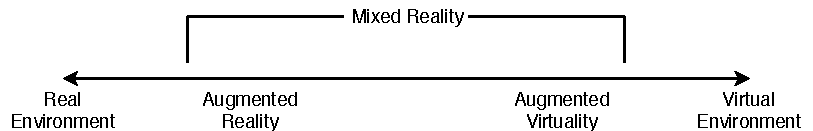
\includegraphics[width=\textwidth]{images/virtualitycontinuum}
	\caption{The Virtuality Continuum}
	\label{fig_mr}
\end{figure}

Mixed reality is often considered as encompassing both augmented reality and augmented virtuality, both of which reside along the ``virtuality continuum'' (see Figure \ref{fig_mr}), a term coined by Milgram and Kishino in 1994  \cite{milgram94}, with the real world at one end and the virtual at the other. Augmented reality refers to an otherwise real world environment in which there can be seen virtual augmentations, often viewed through a clear screen. Augmented virtuality, conversely, attempts to merge real world scenery or objects into an otherwise virtual world.

\subsubsection{Applications and Devices}
The nature of combining real and virtual objects can be utilised in a variety of ways and can enhance a user's ability to perform certain tasks and interact with the world. Whilst initially prevalent in the arts and entertainment industries, mixed reality has a number of practical uses and is being taken advantage of by businesses today, particularly in the fields of military training, manufacturing and education \cite{evans17, hughes97}. Many devices utilise these virtual environments, such as the Oculus Rift and the HTC Vive, headsets that need to be connected to a computer or console, both released in 2016, but the Microsoft HoloLens is one of the few standalone devices available that offers mixed reality capabilities in a head-mounted display.

\subsection{Microsoft HoloLens}
The Microsoft HoloLens is a mixed reality holographic head-mounted display unit with an adjustable cushioned headband released in 2016 \cite{microsoftcorp}. It is ``the first fully untethered holographic computer running Windows 10'', enabling a mixed reality experience with no wires, no external cameras and no connection to a PC required \cite{holmdahl15}.

\subsubsection{Hardware, Sensors and Features}
\begin{table}[!h]
	\renewcommand{\arraystretch}{1.3}
	\caption{Microsoft HoloLens Hardware Specifications}
	\label{hardware}
	\centering
	\begin{tabular}{l|l}
		\toprule
		CPU & Intel Atom x5-Z8100 @ 1.04GHz\\ \hline
		GPU/HPU & HoloLens Processing Unit \\ \hline
		RAM & 2.0GB\\ \hline
		Storage & 64GB\\ \hline
		OS & Windows 10 32-bit\\ \bottomrule
	\end{tabular}
\end{table}
The optics are two separate displays, which are viewed through glass lenses, on to which images are projected and layered to produced what the user can see in their space. The HoloLens' system is essentially mobile hardware (see Table \ref{hardware}) featuring an Intel Cherry Trail Atom chip \cite{rubino16}. Additionally, however, it runs a few processors that make it unique. There is an inertial measurement unit (IMU), which includes an accelerometer, gyroscope, and magnetometer, and there is an aptly named Holographic Processing Unit (HPU), that handles where the user is looking, gesture tracking, spacial mapping and more \cite{holmdahl15}.

It has four ``environment understanding cameras'', two on each side, which provide the basis for tracking the user's head; a depth camera, which helps with hand tracking and performs surface reconstruction (for placing holograms on physical objects); a video camera and an ambient light sensor. These sensors work with the optics module and the IMU and is packaged for the Intel Atom chip by the HPU to produce fast response times to movement so that the user's position is updated and displayed in less than 10ms to ensure the holograms feel part of the world. The HoloLens also features four microphones for receiving user commands, mounted stereo speakers providing spatial sound and both WiFi and bluetooth \cite{colaner16}.

\subsubsection{Practical Applications}
As of 2018 there has only been a few practical applications of the Microsoft HoloLens and a number of them have only been proof of concepts so far. Notably there has been a number of applications developed by NASA in partnership with Microsoft. In 2015 they teamed up for the OnSight and Sidekick projects, utilising the HoloLens on the International Space Station for communication and real-time guidance with ground operators, and later again in 2017 to help find the best places on Mars to build bases \cite{nasa15, microsoftnews17}.

There are also a couple of examples of use in medicine. In 2017 a team of surgeons used the HoloLens to visualise MRI and radiography information whilst operating on a patient with a malignant tumour \cite{bernardo17, 3ders17}. Also in 2017 an ultrasound training simulation was designed to teach healthcare workers proficiency in anatomy through interaction with 3D holograms of internal human structures \cite{lynn17, mahmood17}.

Microsoft are also working on using the HoloLens as a means of communication as part of a research project called Holoportation \cite{cutler17}. Users will have high quality 3D models of themselves rendered in each other's local space. The goal is to allow them to see, hear and interact with one another as if they were in the same room \cite{orts16}.

\subsection{Vuforia}
Vuforia is an augmented reality software development kit designed for Android, iOS and Universal Windows Platform (UWP) applications with support for phones, tablets and eyewear \cite{vuforia, vuforiaeyewear}. The Vuforia engine is natively integrated with the latest versions of Unity and provides the technology to recognise and track images and simple 3D objects in real time. Vuforia provides a developer portal with access to the Vuforia Target Manager that allows the creating and storing of multiple targets to be used by Vuforia applications \cite{vuforiatargetmanager}.

\subsubsection{Target Types}
Vuforia supports a variety of 2D and 3D targets that it stores in databases that it can reference when needing to detect and track objects. These features are listed below:

\begin{table}[!h]
	\renewcommand{\arraystretch}{1.3}
	\caption{Vuforia SDK Features}
	\label{hardware}
	\centering
	\begin{tabular}{c|c|c}
		\toprule
		Images & Objects & Environments \\ \midrule
		Image Targets & Object Recognition & Extended Tracking \\
		Multi-Targets & VuMark & Ground Plane \\
		Cylinder Targets & Model Targets &  \\ \bottomrule
	\end{tabular}
\end{table}

\subsubsection{Related Projects}
There have been a few examples of applications that make use of Vuforia's tracking capabilities to build interactive experiences. These applications tend to be built for mobile devices. In 2014 a mobile advertising application was designed to take advantage of Vuforia's markerless image detection to detect image targets that possessed information relevant to the user \cite{kim14}.

There are far fewer applications that use Vuforia on the HoloLens. In 2017 a simple proof of concept assembly instruction application was attempted in Unity that featured user interfaces, dynamic 3D assembly instructions and spatially registered content placement \cite{evans17}.

\subsubsection{Summary of Findings}
Attempting to capture and manipulate real-world objects on the Microsoft HoloLens is mostly unexplored territory. The HoloLens provides spatial recognition hardware and sensors that allow for head and hand tracking but no built-in object recognition. Vuforia provides the tools to recognise real world objects through the use of a variety of targets stored in the online target databases. The SDK is integrated into Unity and supports development of UWP applications, as well as specifically stating support of the Microsoft HoloLens. 

\newpage
\section{Methodology}
This chapter details the approach taken and the tools that were required during the development of the deliverables. It will describe the work that was undertaken and the problems that arose as a result. The problems encountered ultimately defined the outcome of the deliverables and the ways in which they affected the project are detailed in this chapter.

\subsection{Approach}
There were three principal stages to the development process. The first stage was the project set-up. The second stage details the initial attempts at implementations of object capture using Vuforia's object targets. The final stage was an adaptation to the previous lack of success by changing the implementation to use another target type and later changing the environment in which the detection was desired.

\subsubsection{Stage One: Set-Up}
The first stage was the set-up. This stage included acquiring and getting to grips with the tools and technologies that were to be used. The Microsoft HoloLens was acquired, the required software downloaded and sample projects installed and explored. This stage was important to gain confidence in HoloLens usage and development and allow a more fluid transition to the second stage.

\subsubsection{Stage Two: Object Recognition}
In the second stage the initial attempt to detect real-world objects using Vuforia on the HoloLens was carried out. Vuforia's Object Recognition was chosen as the best targets to use to attempt this given the research done earlier. The additional software required (Vuforia's Object Scanner APK) was installed and an object was scanned in and made a target in Vuforia Target Manager. An application was built using Unity and multiple attempts were made to detect the object, but all were ultimately unsuccessful. This led to the final stage. 
 
\subsubsection{Stage Three: Multi-Targets}
In the final stage of development an adaptation was made and Vuforia's Multi-Targets were explored instead. Images were taken of the multiple sides of a cuboid object and a target was created using Vuforia Target Manager. Another application was built in Unity and more attempts were made to detect the object, but again there was no success. This led to the decision to try to change the environment in which the attempted detection was being made. The project was moved from a bright area with wide windows that provided directional light to a dimmer area with a diffuse overhead light in the hopes that this would enable detection. Both applications were tested and adjustments made but object detection on the HoloLens still didn't occur.

\subsection{Technologies}
The tools that the project required included hardware and software. This included the Microsoft HoloLens, Unity, Visual Studio, Vuforia and its associated tools. The technologies required are detailed below:

\subsubsection{Microsoft HoloLens}
The project was to be developed for the Microsoft HoloLens. The HoloLens was chosen due to its immersive experience when worn, its mixed reality capabilities and its Windows operating system that aligned with Vuforia's support of Universal Windows Platform applications. Microsoft also provide HoloLens Emulator software, however this required a particular version of Windows 10 that the project did not have access to. The University provided the HoloLens for the duration of the project.

\subsubsection{Unity}
Unity is a multi-platform engine with a comprehensive user interface in which immersive applications can be built and features a wide variety of developer tools for 3D virtual environments \cite{unity}. As of Unity 2017.2, Vuforia Engine is delivered as a built-in tool with the majority of the required functionality coming as standard. Unity was used to build the applications that were ran on HoloLens and were primarily composed of Unity's scenes, game objects and cameras.

\paragraph{Scenes}
Scenes provide the environments that the application will run in. It contains the camera for the user view-point, lighting and any game objects required \cite{unityscenes}. Each scene in the applications built during this project were used to house the targets required by Vuforia and the objects to be rendered on those targets as an indication of target detection.

\paragraph{Game Objects}
Game objects are Unity named entities that represent every object used in the scene, including the camera, lighting and the Vuforia targets \cite{unityobjects}. In the applications built these were primarily the camera, any Vuforia targets that were required in the scene, lighting and canvases used for user interfaces.

\paragraph{Camera}
Unity's camera is a required game object that provides the user their field of view and lets them see the environment \cite{unitycamera}. The camera used in this project is a special one provided by the Vuforia SDK that supports augmented reality by removing the background skybox and adjusting the clipping planes to better suit digital eyewear.

\subsubsection{Visual Studio}
Visual Studio is an integrated development environment made by Microsoft. It provides a user interface in which software can be designed, debugged, tested and developed \cite{vs}. For this project Visual Studio will be used to deploy the Unity applications to the Microsoft HoloLens. Applications can be deployed from the development machine to the device over WiFi or via a USB connection. Visual Studio also allows debugging to occur whilst the application is running on the HoloLens.

\subsubsection{Vuforia}
The Vuforia SDK provides the tools to detect and track real world objects through the use of targets. It has a developer portal that allows for easy access to the SDK and associated tools. The tools utilised for the project were Vuforia's Target Manager, Object Scanner and a variety of their pre-defined targets detailed below:

\paragraph{Target Manager}
The Vuforia Target Manager is a tool that allows the creation and management of target databases via the Vuforia developer portal. The databases can be assigned license keys by developers and enables easy management of the targets needed for separate applications. When creating applications users can choose which databases the SDK will use when attempting to detect targets. The tool can also be used to create new targets by uploading images and 3D models to the database and manipulating them to be in-line with the required format for specific targets \cite{vuforiatargetmanager}. 

\paragraph{Image Targets}
Image targets are flat images, such as printed media, that the Vuforia SDK can detect and track. They do not require special black and white spaces or codes to be recognised but instead the SDK tracks features that are found in the image itself by comparing those features against its target resource database. 
Once initially detected the SDK will continue to track the target whilst at least partially in the device camera's field of view and can perform an action or link virtual content to the target \cite{vuforiaimagetargets}, such as the 3D rendered teapot that can be seen in Figure \ref{fig_imagetarget}.

\begin{figure}[!h]
	\centering
	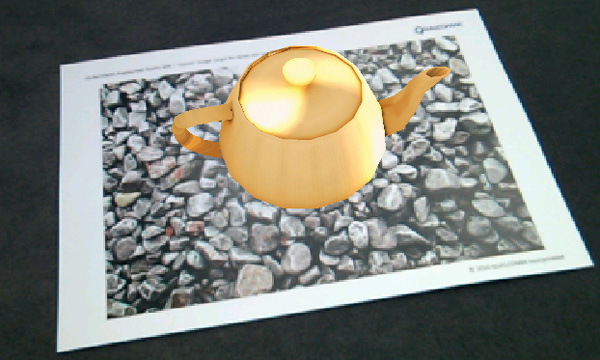
\includegraphics[width=10cm,height=10cm,keepaspectratio]{images/imagetarget}
	\caption[Example Image Target]{An Example Image Target, retrieved from \footnotemark.}
	\label{fig_imagetarget}
\end{figure}

\paragraph{Multi-Targets}
Multi-Targets are created by combining multiple image targets and arranging them into a simple 3D geometric shape, such as a cube. All the faces of a multi-target can be tracked simultaneously as they possess a pre-defined position relative to the target's origin. As a result the entire object can be tracked when any one of its images has been detected  \cite{vuforiamultitargets}. These targets are created by defining a relationship between pre-existing image targets using the Vuforia Target Manager.
\footnotetext{\url{https://vuforialibrarycontent.vuforia.com/Images/devGuide_ImageTargets.jpg}}

\paragraph{Object Recognition and the Vuforia Object Scanner}
Object recognition allows the detecting and tracking of more intricate 3D objects by creating object targets made using the Vuforia Object Scanner. The object scanner is provided as an Android Package (APK), officially it is only supported on the latest Samsung Galaxy devices but can be configured to work on other Android devices \cite{vuforiasupportedversions}. It is an application that can be used to scan a physical 3D object, produces an Object Data (*.OD) file and allows a visualisation of the object target and its coverage. The *.OD file produced by the application can then be uploaded to Vuforia's target manager and an object target created using this data \cite{vuforiaobjectreco}. The SDK will then be able to recognise the real-world object that was scanned by comparing it with the digital representation of the features and geometry that is provided by the object target.

\paragraph{VuMark}

\begin{figure}[!h]
	\centering
	\includegraphics[width=10cm,height=10cm,keepaspectratio]{images/examplevumarks}
	\caption[Example VuMarks]{Example VuMarks, retrieved from \footnotemark.}
	\label{fig_vumark}
\end{figure}

VuMarks are customised markers that encode data and support unique identification and tracking. They are similar to image targets in that they are 2D targets that can be detected and tracked, but provide a lot more that image targets cannot. As the same VuMark design can be used to encode a range of unique IDs or data, they enable the SDK to distinguish between identical looking products using their unique instance ID. VuMarks are designed to enable companies to create augmented reality targets that subtly integrate with their brand \cite{vuforiavumark}, as shown in the example VuMarks in Figure \ref{fig_vumark}\footnotetext{\url{https://vuforialibrarycontent.vuforia.com/Images/Vuforia_6_Images/DesignGuide/ExampleVuMarks.png}}.  

\paragraph{Model Targets}
Model targets enable physical objects to be detected and tracked using a 3D model of the object. The real-world objects are recognised by the Vuforia SDK using a ``specially prepared target database that is generated by processing a digital 3D representation of the object'' using the Model Target Generator tool. Supported objects must be rigid and have matte surfaces. For this to work, the 3D representation of the object should be accurate to a high degree of precision to the physical object. Vuforia's model target test application features a model that is to be 3D printed to be recognised by the SDK \cite{vuforiamodeltargets}.

\subsection{Project Set-Up}
The first stage of work that was undertaken for the project was to acquire the hardware, install the software and begin to get to grips with Microsoft HoloLens development.

\subsubsection{Microsoft HoloLens}
The Microsoft HoloLens was provided by the University for the duration of the project. Initially it required setting-up the device for development, which included creating a Microsoft account, enabling developer mode on the device and ensuring the correct Visual Studio settings were used on the deployment device. It was during this stage that the features and capabilities of the Microsoft HoloLens were explored as part of an attempt to become more familiar with the hardware.

Microsoft provides a comprehensive set of online documents to guide users new to mixed reality development \cite{hololensdev}. It was these guides that were key to the determination of the tools that would be used during the development process of the project. Some of the required tools were downloaded, installed and set up. Initially a basic UWP application was built in Visual Studio and deployed to the HoloLens. This was done to gain a better understanding of how the development machine interacts with the HoloLens and the deployment process.

\subsubsection{Vuforia SDK}
At this stage the focus of the work was on understanding how the Vuforia SDK worked and how to build applications that took advantage of the functionality it supports. During the early stages of development Microsoft's guides recommended that the Vuforia SDK be installed separately and integrated into Unity 5.6 manually. This changed, however, and with the release of Unity 2017.1 the Vuforia Engine was delivered with it.

\paragraph{Vuforia's Samples}
Vuforia provide a comprehensive asset package that can be imported into Unity\footnote{\url{https://assetstore.unity.com/packages/templates/packs/vuforia-core-samples-99026}}. This contains the majority of the default target types, such as image targets, object targets and multi-targets. It also contains a lot of miscellaneous media, such as splash and loading screen images, meshes and materials,  as well as an augmented reality camera object.

Vuforia also provide sample applications for digital eyewear that provide some basic scenes containing example targets\footnote{\url{https://developer.vuforia.com/downloads/samples}}. Much of the steps taken to get these samples running was determined by combining information detailed in the guides provided by Microsoft, Unity and Vuforia. However troubleshooting Vuforia's forums was required as often the guides lacked necessary information. 

The process involved acquiring and applying a Vuforia \textit{Eyewear App License Key} to the Unity project, defining the desired Target Database, fixing the provided camera so that it did not have a skybox and changing the clipping panes to the recommended values for the HoloLens. There were also numerous settings that needed to be changed or enabled in Unity. These included, but are not limited to, enabling virtual reality support in the \textit{XRSettings} in \textit{PlayerSettings}, setting the device type to \textit{Digital Eyewear}, loading the HoloLens Device Config, setting the platform build configurations and enabling extended tracking on each target game object in the advanced section of their behaviour script.  After everything had been correctly configured, and after a not-insubstantial amount of minor changes, the sample could on occasion be successfully deployed to the HoloLens. Even until the very end of development there were certain errors that could appear at different stages that had no discernible pattern or reasoning to their appearance. Troubleshooting only revealed workarounds, such as rebuilding the Visual Studio solution, restarting Unity and, for one particularly inexplicable bug, starting again with a new Unity project and reinstalling the asset packages. This was to be the norm for all subsequent stages of development.

\subsection{Implementation}
\subsubsection{Object Recognition}
At this stage no testing to ensure that Vuforia could detect the simpler targets was undertaken. The downloadable image targets that could be printed off were not used. Instead an attempt at capturing objects using Vuforia's Object Recognition was undertaken.

\paragraph{Choice Over Other 3D Targets}
Vuforia's HoloLens sample contained multiple sample scenes, each showcasing a different target type. One of these was a scene named \textit{ObjectReco} that included the object target as a Unity game object. The decision to begin to attempt object capture using Vuforia's Object Recognition feature rather than its two other 3D targets, VuMark and Model Targets, was twofold. Firstly, using model targets were disregarded earlier due to the constraint of lacking a 3D printer that is required for its functionality. There was also no example scene of model targets provided in the HoloLens sample at the time due to them being relatively new. Secondly, VuMarks were disregarded as they are not true object capture, rather they recognise the 2D VuMark that is applied to a physical object and gather the physical object's information as a result.

\paragraph{Creating an Object Target}
Vuforia's HoloLens sample contained an Object Target game object that was a representation of a Mars habitat. Vuforia provided media that could be printed off and folded such that it would become a physical paper representation of the object target. Since Vuforia provided the tools to create new object targets using the Vuforia Object Scanner and the first goal of the project was to capture real-world objects, the Mars habitat wasn't used.

\paragraph{Vuforia Object Scanner}
Vuforia Object Scanner is provided as an Android Package (APK) and was installed onto an Android device using Android Debug Bridge (adb)\footnote{\url{https://developer.android.com/studio/command-line/adb.html}}. Vuforia also provide an Object Scanning Target\footnote{\url{https://vuforialibrarycontent.vuforia.com/Images/Fall2014/ObjectScanningTarget.PNG}} sheet that was to be printed off and used by the object scanner to determine the position of the Object Target relative to it's local origin.

\begin{figure}[!h]
	\centering
	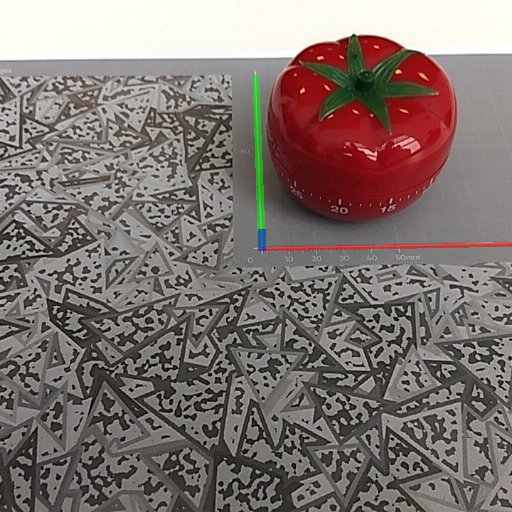
\includegraphics[width=10cm,height=8cm,keepaspectratio]{images/pomo}
	\caption{Pomodoro Timer Object Scanning}
	\label{fig_pomo}
\end{figure}


\paragraph{Scanning}
As seen in Figure \ref{fig_pomo}, the first object chosen to be scanned in was a Pomodoro timer. The origin is the lower left hand corner of the Object Scanning Target's grid region and corresponds to the local (0,0,0) coordinates of the Object Target instance's bounding box. The Pomodoro timer was placed on the grid ensuring none of the outer edges of the object crossed the grid's axes. The object scanner APK uses the Android device's camera to scan the object and starts when the record button is pressed. The device was moved slowly around the object whilst recording, keeping it within view. The APK overlays a simple indication of the object's geometry that is made up of multiple faces that turn green when the corresponding sections have successfully been scanned in. Once the majority of the relevant surface areas were green the recording was stopped and the scanning session was named and the resulting Object Data (*.OD) was saved. The APK provides the capability to test the results of the scan by rendering a green cuboid augmentation at the target's origin when the object is detected. The target was tested in this way against a variety of backgrounds and was successfully recognised as shown in Figure \ref{fig_detection}. 

\begin{figure}[!h]
	\centering
	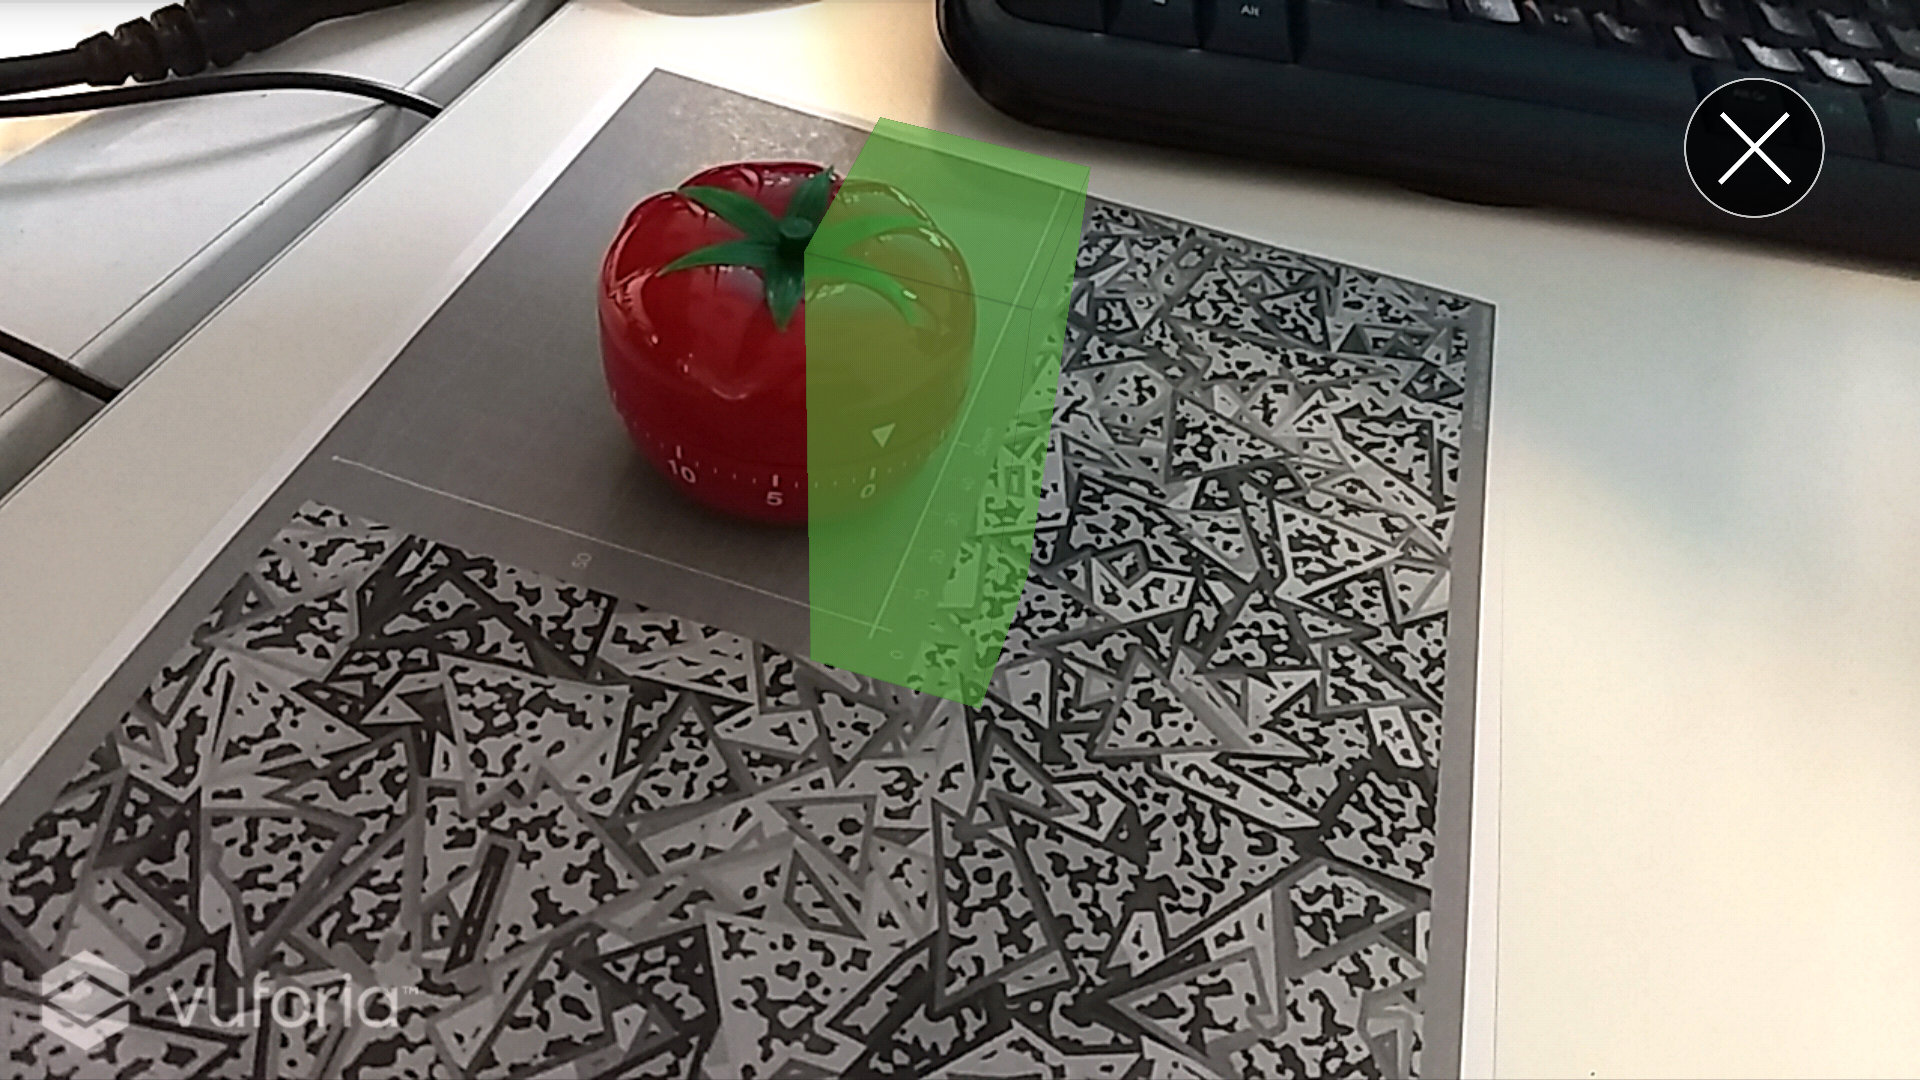
\includegraphics[width=10cm,height=8cm,keepaspectratio]{images/detection}
	\caption[Detection in APK Test]{Object Detection in the APK Testing Feature}
	\label{fig_detection}
\end{figure}

The object data was then sent back to the development machine as an *.OD file. This file was then uploaded to a new target database created for the project using Vuforia Target Manager.

\paragraph{Application}
The Unity project was updated to direct Vuforia to the newly created target database and a new scene was built that contained the ARCamera and the new Object Target. The 3D Mars habitat render was left as the object that would be overlaid and would be used to determine if the Pomodoro timer was successfully detected. The build settings were configured for UWP, the target device set to the Microsoft HoloLens and the debugging option was enabled. The application was exported from Unity into Visual Studio and then built, run and deployed to the HoloLens from there. Despite multiple attempts at reconfiguring the project it was clear the Pomodoro timer could not be detected.

\paragraph{Troubleshooting}
After all the usual guides provided by Microsoft, Unity and Vuforia and their listed solutions to common problems had been exhausted, online forums were turned to in the hope of finding the answers. Quickly it became clear the consensus of other developers was that using Vuforia's Object Recognition tool was very inconsistent when deployed to the Microsoft HoloLens, even the one provided in the sample\footnote{\url{https://developer.vuforia.com/forum/hololens/object-recognition-sample-doesnt-work-hololens}}\textsuperscript{,}\footnote{\url{https://developer.vuforia.com/forum/hololens/improve-object-tracking}}. A Vuforia Support reply on one post suggested that the user wait for the then unreleased Model Target tool\footnote{\url{https://developer.vuforia.com/forum/hololens/object-recognition-unsatisfactory-hololens}}. As so many minor things could affect the success of this object detection method (such as the surrounding environment during the object scanning phase, the material of the object itself and the lighting in the desired detection environment) and there was doubt it could be made to work on the HoloLens at all, it was at this point decided that another type of Vuforia target should be attempted.

\subsubsection{Multi-Target}
Some further research was done into whether anyone had successfully detected real-world objects using Vuforia on the HoloLens and a two-part blog post by Mike Taulty, a Microsoft UK developer, was found \cite{taulty16}. This page (and the previous part) detailed his attempts at simple object recognition using Vuforia's Multi-Targets.

\paragraph{Choice of Target}
Given that the goal was still to capture real-world objects, simply detecting image targets would not be enough. Once again the reasons for not trying Vuforia's other 3D targets, VuMark and Model Targets, were the same. VuMarks were disregarded as not true object capture, and Model Targets as the project did not have access to the 3D printer that they required to be implemented. Multi-Targets can be recognised even if a single child image target is detected and this raised the concern of whether they didn't represent true object capture either, but it was still the closest to the project's goals. As a result it was determined that attempting to capture real-world cuboid objects through the creation of a Multi-Target was to be the next stage of the development. 

\paragraph{Creating a Multi-Target}
\begin{figure}[!h]
	\centering
	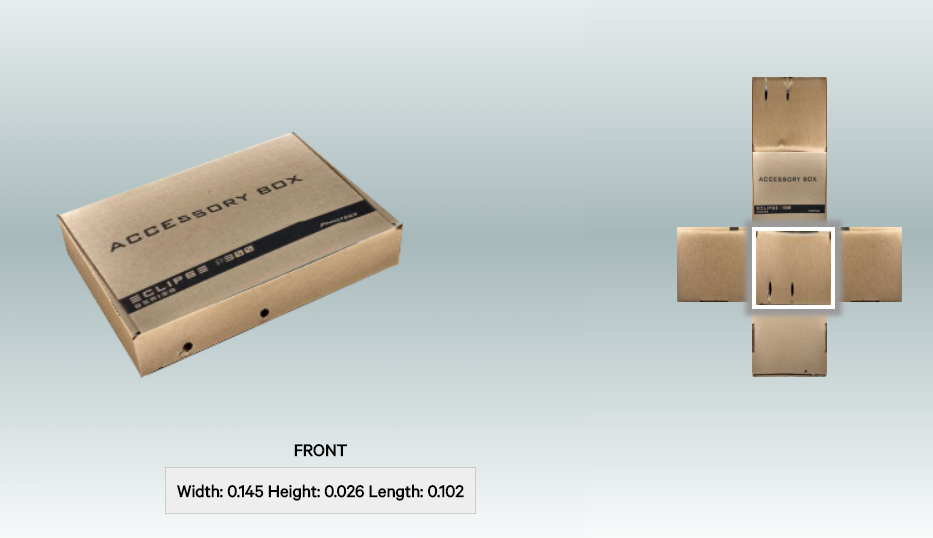
\includegraphics[width=10cm,height=10cm,keepaspectratio]{images/accessorybox}
	\caption[Accessory Box Multi-Target]{Accessory Box Multi-Target in the Vuforia Target Manager}
	\label{fig_accessorybox}
\end{figure}

A multi-target is a Vuforia target that consists of multiple image targets in a defined geometric arrangement. The position and orientation of each image target is defined relative to the Multi-Target's origin and allows the entire target to be detected and tracked whenever one of the child image targets is detected. A Multi-Target was created using the Vuforia Target Manager. A simple cuboid box was chosen and images were captured of each of its faces and uploaded to the manager. The blank mutli-target was built by creating a new target, defining it as a cuboid, inputting its dimensions (in scale with the real box) and then adding it to the previously created target database. At this point the created target could be edited to apply each image to the corresponding face on the virtual cuboid, as shown in Figure \ref{fig_accessorybox}. Meeting the tool's image upload requirements was convoluted: the image needed to be a specific format, under a certain size, and an exact aspect ratio was needed and if it was a pixel off the upload would fail without explanation. 

\paragraph{Application}
Once again the Unity project was updated to reflect the changes represented by the chosen target. The same target database was selected and a new scene was added that contained the ARCamera and the Multi-Target as a game object. This time, a wireframe box that was slightly larger than the Multi-Target object was created, applied to the target and configured so that it would render over the real-world object when detected. This was done so that it would be clear once the application had recognised the box. Once again the application was exported to Visual Studio and deployed to the HoloLens, and once again detection was unsuccessful.

\begin{figure}[!h]
	\centering
	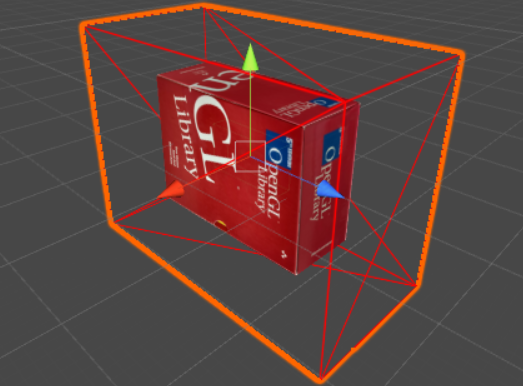
\includegraphics[width=10cm,height=8cm,keepaspectratio]{images/openglbox}
	\caption[OpenGL Box Multi-Target in Unity]{OpenGL Box Multi-Target with Wireframe Cube in Unity Editor}
	\label{fig_openglbox}
\end{figure}

\paragraph{Troubleshooting}
After checking settings and trying to slightly adjust the environments lighting a decision was made to try a different Multi-Target that was richer in detail in the hopes that it could be more easily detected. For the creation of the second target care was taken to ensure there was even lighting on each of the surfaces, no glare was visible and no details of any surface were cut off when the pictures were taken. The target was created in much the same way as before, with the multiple images taken applied to a target with the dimensions of the new box in the Vuforia Target Manager. Shown in Figure \ref{fig_openglbox} is the Multi-Target with its surrounding wireframe box as shown in the Unity Editor. Even with the care taken, there was never any indication of successful object detection. After the usual checks, rebuilding and redeploying, it was determined that a potential underlying issue was the environment in which the object detection was being attempted.

For all the stages of development thus far the work had been undertaken in a wide open room with large floor to ceiling windows on one side that provided the environment with ample daylight. However, this light was noticeably coming from one direction with all objects producing shadows. It also produced glare on otherwise fairly matte objects, such as the second box used to produce a Multi-Target. Given the lack of success it was determined that testing would be taken to a smaller room with less directional light that featured a single overhead light in the hopes of providing a more diffuse light setting. In this new environment each of the previous implementations and all the available 3D targets were tested.

\begin{figure}[!h]
	\centering
	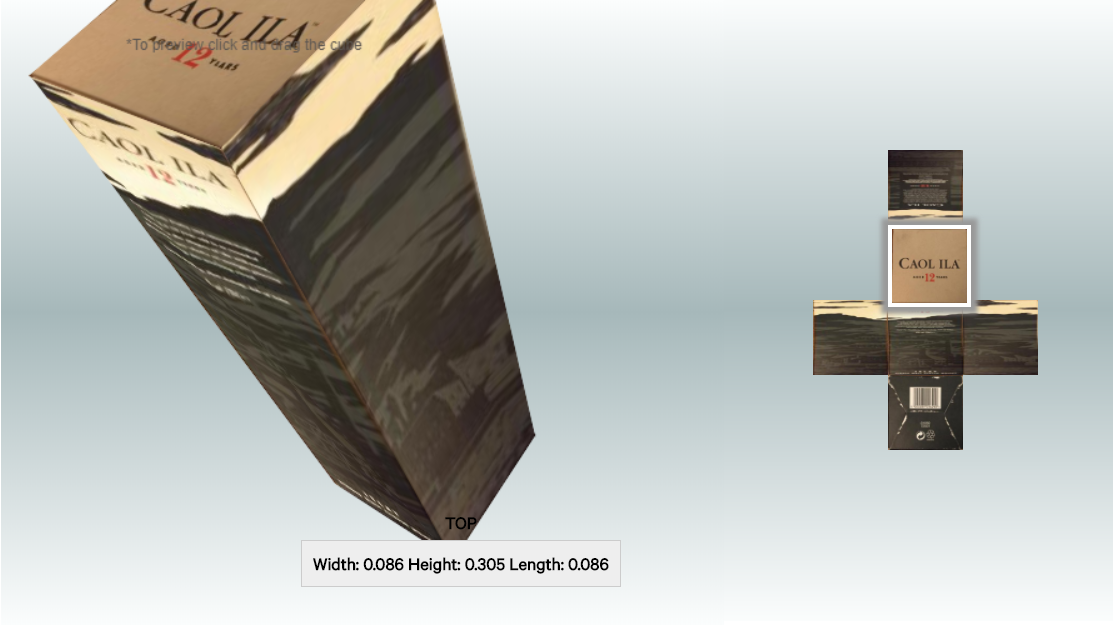
\includegraphics[width=10cm,height=8cm,keepaspectratio]{images/caolila}
	\caption[Whisky Box Multi-Target]{Whisky Box Multi-Target in the Target Manager}
	\label{fig_caolila}
\end{figure}

After multiple attempts at detecting these objects, a third Multi-Target was created using a box that better suited Vuforia's listed requirements for multi-targets. The box chosen was a whisky box as it was rich in detail, made of a matte material, had contrasting regions and none of the sides were the same. The target in its finished form in the Vuforia Target Manager can be seen in Figure \ref{fig_caolila}. Whilst a significant amount of thought and care was put into ensuring an even lighting distribution across each face of the object and a diffuse and well-lit environment the object was still not detected.

\subsubsection{Development Conclusions}
By this stage the development period that was available was coming to a close. A few final attempts were made at detection by changing a number of variables that could have had an affect on the success of the application. The ARCamera's field of view was varied and tested, a range of capabilities in Unity's \textit{Publisher Settings} were enabled and the wireframe box was edited in the hopes that it simply wasn't visible enough before. None of these attempts were successful and the development stage ended without achieving any of the projects initial goals and only delivering some implementations without much functionality.

\newpage
\section{Evaluation}
This chapter looks to evaluate the effectiveness of real-world object capture and real-time object manipulation on the Microsoft HoloLens and to discuss the applicability of the chosen tools. Due to the lack of success at producing any functional applications that could recognise and track simple objects, the project did not progress to the stage of simple object manipulation, let alone real-time manipulations. As a result, there is unfortunately nothing to evaluate in terms of the effectiveness of real-time manipulation of real-world objects. However, the project does allow for a discussion on the effectiveness of real-world object capture, especially with regards to the extent by which it can be achieved on the HoloLens using Vuforia.

\subsection{Object Capture}
When the project was in its infancy, the aim was to capture simple objects in a mixed reality environment whilst using the HoloLens. This was envisioned as detecting and highlighting new objects in real-time. Of course, very early on during the initial research it was realised that such software didn't exist. Instead, via the features provided by the Vuforia SDK, detecting objects required a database of information that can be referenced when scanning the environment for the natural features that make up the target object. Many varied attempts were made, with multiple Vuforia tools and features utilised, but on no occasion was object detection achieved. As a result of the work done in this project it can be said that real-world object capture using Vuforia on the HoloLens is rather ineffective. That statement is also supported by the many others found online, referenced earlier, who were also facing issues when attempting the same. However, there exists examples of projects where a real-world object was detected in space (and augmented such that is was clear the location of the object was being tracked), which was achieved using features provided by Vuforia whilst running on the HoloLens. Whilst these projects did typically utilise Vuforia's VuMarks or Multi-Targets and were not strictly detecting the physical object as a whole, and whilst in one case the author of such a project was a Microsoft developer, they do exist. Therefore, it is worth qualifying that evaluation with an acknowledgement that it is based off of this project's inability to implement such detection rather than a claim that it can't be done.

\subsection{Applicability of the Tools}
All the pertinent tools used for the project were ultimately successful. The results of the initial research done all pointed towards the use of the same few tools and there is good reason for this. Each of the suggested tools fulfilled the purposes for which they were chosen. 

\subsubsection{Visual Studio}
Visual Studio was only used to deploy an application to the HoloLens and occasionally to debug the application whilst it was running. For these purposes, barring occasional build errors usually caused by Unity, it was flawless. Whilst its use time in the project was low, it was a vital part to the development process.

\subsubsection{Vuforia}
The tools Vuforia provide are extensive and, for the most part, fairly intuitive to use. The Vuforia SDK is recommended by Microsoft when wanting to build interactive augmented reality applications and in many respects it is clear why. The features they provide were taken advantage of during development and without which the project would have had very little success. However, there were issues with Vuforia in specific regards to its integration with and operation on the HoloLens. Vuforia's features were much more easily implemented on an Android device. This was shown when the Vuforia Object Scanner used produced an object target that the phone was able to detect very easily. When trying to detect the same object target using the HoloLens very shortly after, there was no such success. There were also problems with a lack of sufficient or reliable documentation available in regards to Vuforia's use with the HoloLens. However, even with the problems, this is technology that is at the forefront of what is capable with the available hardware and no similar object detection software for the HoloLens exists. Given this, Vuforia was an essential tool for the project and will likely continue to be integral for any other project looking at interaction with the real-world in a mixed reality environment. It is worth noting here that at the time of writing many of the guides available online have been updated or rewritten entirely since, as discussed, this is a new technology and is still evolving.

\subsubsection{Unity}
Unity's usage wasn't without issues. Many of the required settings or features that needed to be enabled were not well laid out or easy to find. However it was otherwise a very helpful tool for the project. When it was updated during the project so that it came with the Vuforia SDK integrated, the ease of use when creating these applications was noticeably increased. Beyond that, the tool is very intuitive to use, has good support for the management of multiple Unity projects and was key to the progression of the project as a whole.
 
\newpage
\section{Conclusion}
This chapter is a summary of the findings of the project and details a discussion of whether it met its original goals. It provides a personal reflection on the problems encountered and an overview of what was learned. Additionally, it includes a look at potential work that it could stand to benefit from in the future.

\subsection{Has the Project Met its Aims?}
The main aim of this project was to evaluate the effectiveness of real-world object capture in a mixed reality environment using Vuforia on the Microsoft HoloLens. This has been achieved to some extent in that an evaluation of real-world object capture was possible based on the results of the project and, more specifically, on the lack of success of the implementation. However, it can not be a thorough evaluation as the project did not explore every target type Vuforia allows, nor did it achieve the results that some related projects seem to have achieved. The primary aim of the project was this evaluation and as it was limited by those restrictions the aim was only partially met.

Additionally, however, one of the deliverables this project was looking to develop was an application that allowed users to interact with real-world objects in a mixed reality environment by employing object detection technologies on the Microsoft HoloLens. More than a simple evaluation of the effectiveness of object detection, there was the aim to have a functioning implementation that could showcase object capture in space. This aim was unfortunately not met. All of the implementations produced essentially amount to immersive applications that do not achieve even the simplest of object detection and tracking. This is a disappointing outcome given the scope of the project, the time available and the amount of work undertaken.

As a result of the lack of this initial goal, none of the subsequent milestones, such as simple object manipulation, multiple simultaneous object detection and real-time object manipulation, were even attempted. Manipulation of real-world objects would not have been possible without successful object detection and therefore could not have been implemented. Further to this, the aim to determine the limits of the HoloLens' hardware for the real-time manipulation of multiple real-world objects was left completely unexplored for the same reason.

\subsubsection{Summary of Findings}
In summary, this project was unable to implement any form of real-world object detection in a mixed reality environment using Vuforia on the Microsoft HoloLens. The project did produce a number of other findings that can benefit future development. It did determine that Vuforia's Object Recognition feature is mostly unsupported on the HoloLens despite being part of Vuforia's HoloLens sample project. Successful object detection is usually a result of Vuforia's image detection capabilities, such as VuMarks and Multi-Target, masked as object detection by storing positional data of child targets relevant to the parent object target. The project also highlighted that the full functionality of Vuforia's tools are still in development and undergoing regular improvements. Much of the project's failures can be attributed to the difficulty when creating usable targets. There were many procedures to follow to reduce the chance that a target couldn't be detected with no indication as to what could be causing issues. Ultimately the project found that producing detectable objects using Vuforia's targets on the Microsoft HoloLens was a complex and often convoluted process that unfortunately led to a lack of success regarding the project's aims.

\subsection{Personal Reflection}
This project was in many ways disappointing for me and showed an absence planning and time management. Due to starting development fairly late given the time allotted for the project, many aspects of the work undertaken during the development process were rushed and some more time-consuming potential solutions ignored. This is reflected in the rationale of many of the decisions made during the development process described earlier. I chose not to test the simpler image targets (that could be printed off) provided in the sample projects by Vuforia as they weren't pertinent to the goal of capturing real-world objects. I chose not to explore Vuforia's Model-Targets due to not having a 3D printer, but there may have been ways to gain access to such a device if its need had been realised earlier. There are also a number of more minor mistakes that can be seen, such as using an object that produces a noticeable amount of glare when creating an Object Target. This meant the position of the object needed to be the same during detection testing as it was when the target had been created.

To produce a successful piece of work of this magnitude demands proper forethought and a real attempt at sticking to a plan of work throughout. The lack of this is in my project is clear. Whilst plans were drawn out on multiple occasions, following through with more than the plan's first step rarely happened. The fact that the majority of the development process didn't begin until such a stage that what was done was rushed is evidence of this. My tendency to do work in this manner is what causes shortcomings in all my projects and can  only be amplified for a project of this scale.

Nonetheless I feel there are aspects of the project that I can be proud of. I had the ability to work hard when needed to. I was able to produce a thoroughly researched background of the technology that underpinned the the rest of the development. I also produced a well-reasoned evaluation of the outcomes of the project, with respect to the initial goals and to related work, and of the tools used. 

\subsubsection{Learning Outcomes}
\paragraph{L.O.1: Manage a substantial individual project, including planning, documentation and control.}
I showed a somewhat limited ability to manage this project, thorough planning was missing and abiding by the time constraints was mostly unsuccessful. However, there was still an amount of work undertaken and findings produced to show some success in the management of a substantial individual project, including completing the required documentation to a high standard.

\paragraph{L.O.2: Construct a focussed problem statement and conduct a suitable investigation, including literature or technology review, into the context of that problem.}
The problem the project sought to address was well-reasoned and provided a clear set of relevant milestones. The technological review was thorough and applicable to the problem discussed as well as providing the foundations upon which the project was carried out.

\paragraph{L.O.3: Demonstrate professional competence by applying appropriate theory and practice to the analysis, design, implementation and evaluation of a non-trivial set of deliverables.}
The steps taken and outlined in the methodology display thoughtful analysis of the problems at hand and a logical process by which I sought to solve them. Unfortunately due to there being no successful implementation deliverable this was not done as well as I could have hoped. The evaluation of the results of the project were appropriately qualified and supported with evidence.

\paragraph{L.O.4: Show a capacity for self-appraisal by analysing the strengths and weaknesses of the project process and outcomes with reference to the initial objectives and to the work of others.}
I made a real attempt to adequately criticise myself for my failures but also to highlight aspects worth praising. I also compare my findings to related work and to the initial goals of the project.

\paragraph{L.O.5: Provide evidence of the foregoing in the form of a report.}
I completed the project's documentation successfully, including evidence of having at least partial achievement for all the previous learning outcomes, and fulfilling all the requirements laid out for the dissertation and its formatting specifications.

\subsection{Future Work}
The work that can still be done on this project is substantial. A variety of avenues for success were not explored and many of the milestones were not attempted.
\subsubsection{Object Detection}
The primary goal for the future would be to produce a more professional object target creation environment. By building a scene with even surroundings and lighting using a setting similar to those used in photography studios, the target's specific recognition data would be better produced. This is something that would likely significantly increase the chance of object detection and allow for detection in variety of environments.

The next stage this project would have explored was Vuforia's Model-Targets. These were previously dismissed due to lacking a 3D printer which was required for functionality. Additionally capturing a physical object that was simply a 3D print of the virtual model seemed initially less in line with the project's goals. However given detection was yet to occur, this would be the next logical tool to explore. 

Another of Vuforia's tools for object detection is VuMark. Using these the object geometry data can be retrieved from the database and used to produce same-size virtual content in the place of the real-world object on which the VuMark is placed. VuMarks should allow for better consistency with detection as well due to the more unique patterns they employ, similar to QR codes.

\subsubsection{Object Manipulation}
As is in line with the initial project goals, another path that could be taken is one which would have been explored had object detection and tracking occurred. Once an object can be reliably recognised and a 3D render of that object put in its place, multiple simple post-processing effects could be applied to manipulate the object's appearance. Expanding on this, the tools to choose what manipulations are applied and having these manipulations occur in real-time on a variety of desired objects could be built. By providing this, the goal of producing a tool that allows a user to interact and manipulate their local space could be achieved.

At this stage the project could benefit from an analysis of the capabilities of the Microsoft HoloLens' hardware. Tests could be run to determine to what extent manipulations can happen in real-time and on how many objects. This would be carried out by testing the amount of time taken to produce the successful manipulation and an evaluation of whether this is considered real-time done by performing a user study.

\subsubsection{Technological Application}
As a result of the potential work detailed here, the technology could be developed to the stage where it can be used by others in ways similar to those described in the project's motivation. There could also be a number novel ways to use the technology for creative endeavours. Objects could be made to grow or shrink in space, or to seemingly disappear altogether. The project could also provide the basis for a detailed story-driven game that requires interaction with the real-world but augmented by the virtual.

\newpage
\begin{singlespace}	
\bibliographystyle{IEEEtran}
\bibliography{Bibliography}
\end{singlespace}

%example of References. See https://en.wikibooks.org/wiki/LaTeX/Bibliography_Management
%might be good to use a separate document for these so your main work is not one really long text file. 

%you can crate this on a extra tex document just like the title or any other part of the document.
\newpage
\begin{appendices}
\section{Initial Project Overview}
\textbf{SOC10101 Honours Project (40 Credits)} \\ \\
\textbf{Title of Project:} \\
Real world object-capture in a mixed-reality environment. \\ \\
\textbf{Overview of Project Content and Milestones:} \\
This project will look to evaluate the effectiveness of capturing real world objects using Vuforia on the Microsoft HoloLens. Initially, a method to capture a simple object will be developed, before attempts to capture more complex (or multiple) objects and real-time object manipulation will be implemented. The project aims to explore to what extent this can be done. \\
The milestones will be: 
\begin{itemize}\itemsep0pt
	\item simple object capture
	\item simple object manipulation
	\item complex object capture
	\item real-time object manipulation.
\end{itemize}
\textbf{The Main Deliverable(s):} \\
Object capture and manipulation software. \\
Dissertation. \\
Poster. \\ \\
\textbf{The Target Audience for the Deliverable(s):} \\
Technical mixed-reality game developers looking for new game mechanics. \\
Enthusiasts interested in new game technologies. \\ \\
\textbf{The Work to be Undertaken:} \\
Research similar attempts at mixed-reality object manipulation. \\
Design a method to capture a cube (or similar object) using Vuforia. \\
Build and apply simple shaders to the object. \\
Expand on above methods to capture more complex objects. \\
Explore and evaluate the extent to which the objects can be manipulated in real-time. \\
Document and report findings. \\ \\
\textbf{Additional Information / Knowledge Required:} \\
Creating and managing Unity projects. \\
How to use Vuforia. \\
Improve understanding of shader usage. \\ \\
\textbf{Information Sources that Provide a Context for the Project:} \\
General Development Page for the HoloLens: \\
\url{https://developer.microsoft.com/en-us/windows/mixed-reality/development} \\
Some related downloadable tools: \\
\url{https://developer.microsoft.com/en-us/windows/mixed-reality/install_the_tools} \\
Vuforia Specific: \\
\url{https://developer.microsoft.com/en-us/windows/mixed-reality/vuforia_development_overview} \\
\url{https://developer.vuforia.com} \\ \\
\textbf{The Importance of the Project:} \\
Mixed-reality is an emerging games technology with great potential for immersive story-telling and innovative game design. This project looks to explore an aspect of that and if successful could be beneficial to those interested in designing such games. \\ \\
\textbf{The Key Challenge(s) to be Overcome:} \\
Lack of similar projects documented. \\
Fairly niche/specialist/obscure software, mostly new territory. 
\newpage

\section{Report on the Interim Review Meeting}
\ \\ \textbf{SOC10101 Honours Project (40 Credits)} \\                   
\textbf{Week 9 Report} \\ \\
\textbf{Student Name:} Beej Persson \\
\textbf{Supervisor:} Kevin Chalmers \\
\textbf{Second Marker:}  Gregory Leplatre \\
\textbf{Date of Meeting:}  20/11/2017 \\
Can the student provide evidence of attending supervision meetings by means of project diary sheets or other equivalent mechanism?  \textbf{no*} \\
\indent If not, please comment on any reasons presented \\
\textsl{No evidence provided but no indication from supervisor that there was a problem with weekly meeting attendance.} \\ \\ \\
Please comment on the progress made so far \\ \\
\textsl{The work done focused on identifying ways of working with a Hololens, i.e., the output side of the project. This was useful, but the main challenge of the project is object recognition and augmentation, which would have been useful to deal with earlier. This would also have allowed you to engage with relevant literature on the subject.} \\ \\ \\
Is the progress satisfactory? \textbf{unsure} \\
Can the student articulate their aims and objectives? \textbf{Partly} \\
If yes then please comment on them, otherwise write down your suggestions. \\ \\
\textsl{The overall goal (altering the appearance of real-world objects using AR) is clear. What specific alterations, to which objects and in which context remains to be determined. Familiarity with relevant literature will help you specify your project more accurately. Many things are possible, some more complex than others. For this type of project, a good approach would be to consider what operation would have the highest visual impact while having a manageable development cost. There is definitely potential in your project.} \\ \\ \\	
Does the student have a plan of work? \textbf{Yes} \\
If yes then please comment on that plan otherwise write down your suggestions. \\ \\
\textsl{Unfortunately, the plan is limited to work already done.} \\ \\ \\
Does the student know how they are going to evaluate their work? \textbf{partly} \\
If yes then please comment otherwise write down your suggestions. \\ \\
\textsl{The proposed approach is sensible but it is difficult to be more specific at this stage as the functionalities of the system aren’t clearly defined.} \\ \\
Any other recommendations as to the future direction of the project \\ \\
\textsl{With Vuforia, you should be able to capture objects in a scene (in advance) and then track these objects. The acquisition/tracking effectiveness probably depends on the complexity of the object, which you should establish. Once you know the limits of what you will be able to track, you can focus on real-time alterations. Your incremental development approach is suitable, but it needs to be better controlled. Once you know what you are aiming to do, you can define the incremental steps that will lead you there. The core of the research in this area is about achieving realism, which involves lighting and material acquisition. Potentially impactful results can also be achieved by taking slighting different directions. Giving an object a stylised look is one of them. Anecdotally, magic tricks are high impact and can be technically cheap. A magic trick you could implement could be: give a physical object to a user (that you will have previously scanned with Vuforia). Ask them to put it on a table (that you have also previously scanned), and make the object disappear (assuming the user is wearing a Hololens).} \\ \\
\begin{tabbing}
	Signatures: \hspace{1em} \= Supervisor \hspace{2em} \= Kevin Chalmers \\
	\> Second Marker \> Gregory Laplatre \\ \\
	\> Student \>
\end{tabbing}
Please give the student a photocopy of this form immediately after the review meeting; the original should be lodged in the School Office with Leanne Clyde
\newpage
\end{appendices}

\end{document}
